%% This LaTeX-file was created by <wiera> Thu Aug 10 15:33:22 2000
%% LyX 0.12 (C) 1995-1998 by Matthias Ettrich and the LyX Team

%% Do not edit this file unless you know what you are doing.
\documentclass[a4paper,english]{report}
\usepackage[T1]{fontenc}
\usepackage[latin1]{inputenc}
\usepackage{babel}
\usepackage{graphics}

\makeatletter


%%%%%%%%%%%%%%%%%%%%%%%%%%%%%% LyX specific LaTeX commands.
\newcommand{\LyX}{L\kern-.1667em\lower.25em\hbox{Y}\kern-.125emX\spacefactor1000}

%%%%%%%%%%%%%%%%%%%%%%%%%%%%%% Textclass specific LaTeX commands.
\newenvironment{lyxcode}
  {\begin{list}{}{
    \setlength{\rightmargin}{\leftmargin}
    \raggedright
    \setlength{\itemsep}{0pt}
    \setlength{\parsep}{0pt}
    \ttfamily}%
   \item[]}
  {\end{list}}

%%%%%%%%%%%%%%%%%%%%%%%%%%%%%% User specified LaTeX commands.
\usepackage{textcomp}
\makeatother

\begin{document}


\title{Diploma Thesis:\\
Utility Support for Checking OCL Business Rules in Java Programs}


\author{Ralf Wiebicke}


\date{May 2000}

\maketitle

\section*{Copyright}

Copyright \copyright~2000 Ralf Wiebicke.

Permission is granted to copy, distribute and/or modify this document under
the terms of the GNU Free Documentation License, Version 1.1 or any later version
published by the Free Software Foundation; with no Invariant Sections, no Front-Cover
Texts, and no Back-Cover Texts. A copy of the license is available at http://www.gnu.org/copyleft/fdl.html.

The source code developed together with this paper is Copyright \copyright~2000
Ralf Wiebicke and published under the GNU Lesser General Public License.


\section*{Availability}

This document is available at http://dresden-ocl.sourceforge.net/diploma\_rw7/
in several electronic forms including \LaTeX{}, Postscript, PDF, Html and the
original kLyx version. 

The source code developed together with this paper is available at http://dresden-ocl.sourceforge.net/.

\tableofcontents


\chapter{Introduction}


\section{OCL and Extreme Programming}


\chapter{Code Generation}


\section{Representation Of Associations}


\subsection{Possibilities}

\begin{itemize}
\item Collections named by the role name (maps for qualified associations)
\item Methods (isEmployed)
\end{itemize}

\subsection{CASE-Tools}


\subsection{Net-Linx}

adaptability to legacy Quellcode.


\section{Model Information\label{Sec:element_type_tag}}

The OCL compiler needs model information for type checking. How this works is
explained in \cite{ff3} section 5.3.3. The sources for model information may
be a UML model exported from a CASE tool, or the java source code, which is
accessed through reflection API\footnote{
see class \texttt{tudresden.ocl.check.types.ReflectionFacade}.
}. The latter approach is very convenient, since most java projects don't have
a (up to date) UML representation of their business model. 

However, java reflection lacks some model properties which are important for
type checking.

\begin{enumerate}
\item Element types of collections, particularly collections representing associations. 
\item Qualifier types of maps, representing qualified associations.
\item The isQuery tag of operations. Note, that OCL expressions may use operations
without side effects (queries) only.
\end{enumerate}
The solution is to put the additional information needed into java documentation
comments. See the example below. 

\begin{lyxcode}
class~Company\\
\{\\
~~/{*}{*}\\
~~~~~All~persons~employed~by~this~company.\\
~~~~~@element-type~Person\\
~~{*}/\\
~~Collection~employees;\\
\}
\end{lyxcode}
The new \texttt{@element-type} tag has a syntax like \texttt{@see} as defined
in \cite{JAVA} section 18.4.1, but may refer to classes and interfaces only.
This tag is valid for attributes only, and there may be only one of such tags
per documentation comment. The tag is not restricted to attributes of type \texttt{java.util.Collection},
since future implementations could use other collection API's as well.

Analogously, the \texttt{@key-type} tag is introduced for association qualifiers. 

\begin{lyxcode}
class~Bank\\
\{\\
~~/{*}{*}\\
~~~~~Customers~qualified~by~their~account~number.\\
~~~~~@element-type~Person\\
~~~~~@key-type~Integer\\
~~{*}/\\
~~Map~customers;\\
\}
\end{lyxcode}
Note, that the reflection model is restricted to qualified associations with
one qualifier only. \cite{UML} allows multiple qualifiers, but there is no
convenient representation for this in java. 

Furthermore, UML specifies the unqualified association feature to be a set,
i.e. there must be no duplicates. Since this is not enforced by \texttt{java.util.Map}
(only keys are guaranteed to be unique), the injector provides an appropriate
runtime check.


\paragraph{Implementation.}

A really comfortable implementation would let the java compiler do the parsing,
and provide the information through an extended reflection API. This would be
similar to the \texttt{@deprecated} tag. My implementation extends\footnote{
Encapsulated in \texttt{tudresden.ocl.check.types.ReflectionExtender}.
} the reflection facade by scanning the source code for these comments on demand.
This implies, that the java source code is necessary for type checking OCL constraints
in addition to the class files.

There is a crucial question left: Where do the tags come? Possible sources are:

\begin{itemize}
\item A UML model. The code generator of a CASE tool could generate these tags. 
\item Maintained by hand. It is good-practice of programming, to specify which kind
of objects are supposed to be in a collection attribute. The tags just make
this information available formally. 
\item Reverse Engineering. This is discussed in detail in chapter \ref{Sec:ReverseEngineering}.
\end{itemize}
Collection attributes with type tags are verified on runtime by the injected
code. Note, that this kind of type information is useful for reverse engineering
a UML model from given java code.


\section{Looking at Previous States}

only 1 @pre pro navigation, may be proposal


\chapter{Code Injection}

Injection of generated code into java programs is the main subject of this paper.
It covers anything beyond code generation, to get a java model checking its
own constraints. For an idea, where code generation ends and injection starts,
see section \ref{Sec:codegeneration_result}. 

This is followed by an analysis of requirements for the code injection and resulting
design decisions in section \ref{Sec:injection_requirements}. Sections \ref{Sec:wrappingMethods}
and \ref{Sec:cleaningCode} describe the solution in detail.

Finally sections \ref{Sec:temporalScope} and \ref{Sec:structuralScope} discuss
the more fundamental issue, when and how often invariants have to be checked.


\section{Results of Code Generation\label{Sec:codegeneration_result}}

The java code generator developed in \cite{ff3} produces a set of code fragments\footnote{
see class \texttt{tudresden.ocl.codegen.CodeFragment.}
}. These code fragment have the following properties:

\vspace{0.3cm}
{\centering \begin{tabular}{|l|p{70mm}|}
\hline 
Property &
\\
\hline 
\hline 
Constrained~type &
The default navigation context of this constraint.\\
\hline 
Kind &
Specifies, whether this constraint is an invariant, a pre- or a postcondition.
\\
\hline 
Constrained~operation &
The operation, this constraint applies to (valid for pre- and postconditions
only).\\
\hline 
Code &
Contains the actual java code to be executed.\\
\hline 
Result~variable &
Specifies the boolean value, which contains the result of the ocl expression
after code execution.\\
\hline 
\end{tabular}\par}
\vspace{0.3cm}

For each postcondition containing a @pre expression there are two additional
codefragments called preparation and transfer. See below.


\subsection{Preparation and Transfer Fragments}

The meaning of preparation and transfer fragments is explained on a dramatically
simplified example. 

Suppose a post condition for operation \texttt{employ()}, that leaves the attribute
\texttt{age} unchanged:

\begin{lyxcode}
context~Person::employ()~\\
post:~age=age@pre
\end{lyxcode}
the following codefragments will be produced:

\vspace{0.3cm}
{\centering \begin{tabular}{ll}
\hline 
Kind&
 Code\\
\hline 
\hline 
Transfer&
\texttt{int~node1;} \\
\hline 
Preparation&
\texttt{node1=this.age;}\\
\hline 
Post Condition&
\texttt{int~node2=this.age;}\\
&
\texttt{boolean~result=(node1==node2)}\\
\hline 
\end{tabular}\par}
\vspace{0.3cm}

Typically these fragments would be injected as follows:

\begin{lyxcode}
class~Person\\
\{\\
~~void~employ()\\
~~\{\\
~~~~int~node1;~~~~~~~//~transfer~fragment\\
~~~~node1=this.age;~~//~preparation~fragment\\
~~~~//~original~code~of~employ()\\
~~~~//~post~condition~fragment\\
~~~~node2=this.age;\\
~~~~boolean~result=(node1==node2)\\
~~\}\\
\}
\end{lyxcode}
Note, that precise semantics of codefragments involving the @pre expression
has been changed, so that the original meaning described in \cite{ff3} section
7.1.2 is no longer fully correct. For a detailed comparison see section \ref{Sec:maintainJavaCodeGenerator}.

\begin{lyxcode}
~
\end{lyxcode}

\section{Requirements and Design Decisions\label{Sec:injection_requirements}}

This section analyzes the requirements for the injector tool and derives some
fundamental design decisions.


\subsection{Reversable Modification\label{Sec:injection_requirements_reversable}}

The most important feature is the reversability of the code injection. It must
be possible

\begin{itemize}
\item to clean the code tracelessly from all injected fragments.
\item to redo the injection on source code that has already been modified (i.e. when
constraints have been changed).
\item to edit the modified source code without losing all changes at the next injection. 
\end{itemize}
This requirement makes things quite a bit more difficult, but there are serious
reasons for this. Otherwise there would be two versions of source code: the
original and the modified version. This raises some unpleasant problems:

\begin{enumerate}
\item Configuration management must handle two source code trees.
\item Developers must be careful to edit the original version only.
\item Running the ocl injector is required after every change of the java source code,
not only when the constraints have been changed. 
\item Stack traces of runtime exceptions point to the modified source code. Developers
must look for the corresponding place in the original version.
\end{enumerate}
The implementation of reversable modification requires a strategy of minimally
invasive modification. This is realized by two design decisions:

\begin{enumerate}
\item Method wrappers, explained detailed in section \ref{Sec:wrappingMethods}.
\item Explicit package qualifiers for the ocl library in the generated code. Otherwise,
an import statement for the ocl library would be necessary. This would be just
another spot, were the original source code had to be touched. Additionally,
this may introduce name conflicts beetween ocl library and user code.
\end{enumerate}

\subsection{Embedding Constraints in Java Source Code.}

It should be possible to embed constraints in the java documentation comments.
The placement of embedded constraints implicates (and replaces) the context
of the constraint. See the example below.

\begin{lyxcode}
/{*}{*}\\
~~~@invariant~age>0\\
{*}/\\
class~Person\\
\{\\
~~int~age;\\
~\\
~~/{*}{*}\\
~~~~~@postcondition~age=age@pre\\
~~{*}/\\
~~void~employ();\\
\}
\end{lyxcode}
It is necessary to put the constraints directly under the nose of the developer.
The author is strongly convinced, that constraints stored in an extra text file
are too far away from attention.

This feature is not implemented yet. TODO.


\subsection{Checking the Element Type.}

The injected code must check, that collection attributes comply to the \texttt{@element-type}
and \texttt{@key-type} tags introduced in section \ref{Sec:element_type_tag}.
This is quite easily done just before checking invariants.

Note, that this feature may be be used standalone, without ocl expressions at
all. Then it provides a runtime check for typed collections.


\section{Methods Wrappers\label{Sec:wrappingMethods}}

The main task of code injection is to have some code executed immediately before
and after all methods (and after all constructors too). This section describes,
how this is done by the ocl injector.


\paragraph{Simple Approach.}

The simple approach of adding the code directly into the method raises some
severe problems. 

\begin{enumerate}
\item The postcondition code to be executed after the method has to be inserted at
any return statement.
\item A return expression has to be computed in advance, if the post condition code
refers to the return value and/or the the return expression produces side effects.
\item There may be name conflicts beetween the original and the generated code.
\item A complete java parser is needed.
\item The original code has to be touched at many different places and in a complicated
way. This runs contrary to the strategy of minimally invasive modification as
decided in section \ref{Sec:injection_requirements_reversable}.
\end{enumerate}
Method wrappers solve all these problems in a nifty but simple way.


\paragraph{Wrapping Methods.}

Some code tells more than thousand words, so I use an example to explain. Consider
the following method.

\begin{lyxcode}
int~someMethod(double~x)\\
\{\\
~~//~here~comes~the~code.\\
\}~
\end{lyxcode}
The code injector transforms this into two methods.

\begin{lyxcode}
int~someMethod\_wrappedbyocl(double~x)\\
\{\\
~~//~here~comes~the~code.\\
\}\\
~\\
int~someMethod(double~x)\\
\{\\
~~//~some~code~checking~invariants/preconditions.\\
~~int~result=someMethod\_wrappedbyocl(x);\\
~~//~some~code~checking~invariants/postconditions.\\
~~return~result;\\
\}
\end{lyxcode}
The reader may have a look back at the problems encountered for the simple approach.
Non of them exists anymore. Especially, a very inchoate java parser is sufficient,
which understands anything outside of method bodies and attribute initializers
only.


\paragraph{Wrapping Constructors.}

Another transformation is used for constructors, since they cannot be renamed.

\begin{lyxcode}
SomeClass(String~x)\\
\{\\
~~//~here~comes~the~code\\
\}
\end{lyxcode}
Instead of renaming, the original constructor gets an additional dummy argument.

\begin{lyxcode}
SomeClass(String~x,~Dummy\footnote{
actually this is class \texttt{tudresden.ocl.injection.lib.WrapperDummy}.
})\\
\{\\
~~//~here~comes~the~code\\
\}\\
~\\
SomeClass(String~x)\\
\{\\
~~this(x,~(Dummy)null);\\
~~//~some~code~checking~invariants.\\
\}
\end{lyxcode}
If a class provides no explicit constructor, then there is the default constructor
as specified in \cite{JAVA} section 8.6.7. This default constructor is not
wrapped, but replaced by an explicit constructor with the same access modifier.


\section{Cleaning the Code\label{Sec:cleaningCode}}

Reversable modification means, that the injector is able clean the modified
code without leaving any traces. This section explains, how this requirement
is met. 

The user code is modifies in two different ways only:

\begin{enumerate}
\item Renaming the wrapped methods/constructors.
\item Adding new object features, i.e. wrapper methods, methods for checking invariants
and observing attributes.
\end{enumerate}

\paragraph{Renaming Wrapped Methods.}

For each method to be wrapped the suffix \texttt{\_wrappedbyocl} is appended
to the name. This transformation is done on the unparsed method header, so all
typographical extras (line breaks, comments etc.) are preserved. This transformation
is easily reversed, when the code has to be cleaned. For constructors, this
works similarly with appending the dummy parameter to the parameter list.


\paragraph{Removing Generated Features.}

Removing generated class features relies on the fact, that the injector tags
all generated features as shown below.

\begin{lyxcode}
/{*}{*}\\
~~~@author~ocl\_injector\\
{*}/\\
void~checkOclInvariants();
\end{lyxcode}
When cleaning the code, the injector simply removes all object features carrying
such an \texttt{@author} tag. This is quite simple and functional.


\section{Scope of Invariants\label{Sec:temporalScope}}

This section discusses the issue, when an invariant is required to be fulfilled.
\cite{Warmer} section 5.4.2 suggests to check invariants immediately after
an object has changed. This is not workable, even if runtime efficiency is ignored.
Modifications on the model often produce intermediate states, which are not
consistent according to the constraints.

When using databases the answer is simple: invariants must be valid outside
of transactions. Since the java system does not provide transactions, the code
injector offers several strategies for various user requirements.

Invariants may be required to be fulfilled on:

\begin{itemize}
\item All methods. This may be too strict, since private methods may intentionally
leave an object in an inconsistent state. 
\item Public methods (or any other access modifier). This may be not strict enough.
\item Tagged methods. A special tag in the documentation comment declares, that a
method promises to leave the system in a consistent state. This tag is then
part of the interface contract. This is the best solution, but requires additional
effort spent by the developer.
\item Explicit request. This is the way of choice, if the model is held in a database
backend. Then the checking of invariants is simply done immediately before committing.
\end{itemize}
These strategies may used in conjunction. Except of \emph{All Methods} together
with \emph{Public Methods} and/or \emph{Tagged Methods} all other combinations
make sense for special user requirements.

The current implementation does not yet provide tagged methods. TODO.


\section{Caching Results of Invariants\label{Sec:structuralScope}}

The previous section discussed, when we have to make sure, that all invariants
are fulfilled. But even then it's not absolutely necessary to evaluate all invariants.
The implementation developed along with this paper checks only those invariants,
whose result may possibly have changed by recent changes of the model.


\subsection{Design}

Caching is realized with an observer design. Each invariant determines all object
attributes it depends on and registers to these attributes as observer. Figure
\ref{Abb:observingInvariants} shows the meta model of the principal design.

\begin{figure}
{\centering \resizebox*{1\columnwidth}{!}{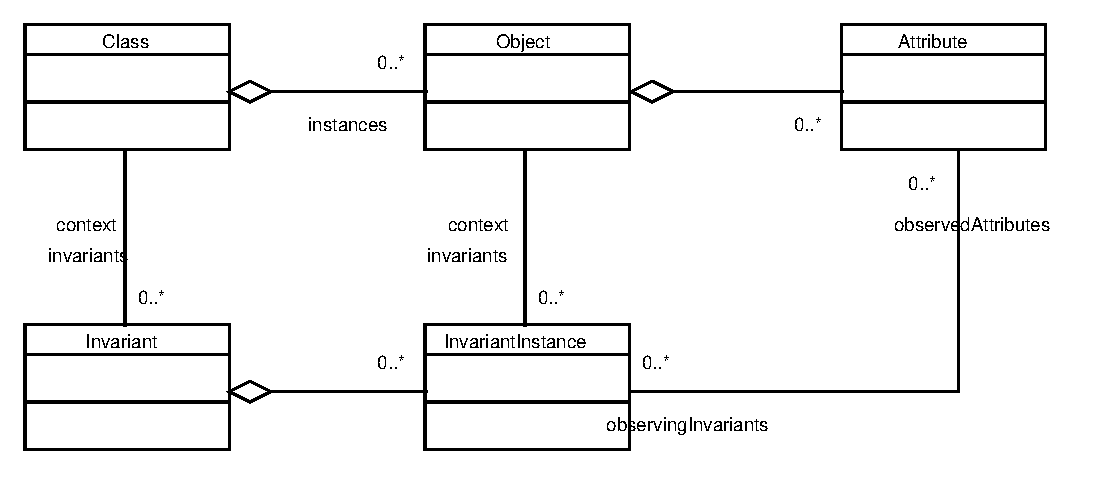
\includegraphics{observingInvariants.eps}} \par}


\caption{Design for Observing Invariants\label{Abb:observingInvariants}}
\end{figure} 

The classes in the UML chart have the following meaning:

\vspace{0.3cm}
{\centering \begin{tabular}{|l|p{5cm}|p{3cm}|}
\hline 
Class&
&
Example\\
\hline 
\hline 
Class&
An arbitrary class of the user model&
\texttt{class~Person}\\
\hline 
Invariant&
An invariant in the context of a class&
\texttt{context~Person~inv:~age>=0}\\
\hline 
Object&
An instance of a class&
Person ``Smith''\\
\hline 
InvariantInstance&
An invariant in the context of an object.&
Has ``Smith'' a positive age?\\
\hline 
Feature&
A feature (attribute or query method) of an object.&
\texttt{Person.age}\\
\hline 
\end{tabular}\par}
\vspace{0.3cm}

For now, lets think of features as attributes only. How to deal with query methods
is explained below. 

The cycle of checking invariants contains two stages.

\begin{enumerate}
\item Evaluating invariants. When evaluating an invariant instance, this invariant
instance registers to all object attributes used during evaluation as observer.
This means, the attribute promises to notify the invariant instance, when the
attributes value changes.
\item Running the model. When an attribute changed its value during execution of user
code, it notifies all observing invariant instances. Then, the attribute unregisters
all observers, so they must register again on the next evaluation stage.
\end{enumerate}
This design can be extended to query\footnote{
Operations used in ocl expressions must not have side effects.
} methods. If the query does not have parameters, it's exactly like attributes.
Things get a bit more complex, if the queries are parameterized. See figure
\ref{Abb:observingMethods}.

\begin{figure}
{\centering \resizebox*{1\columnwidth}{!}{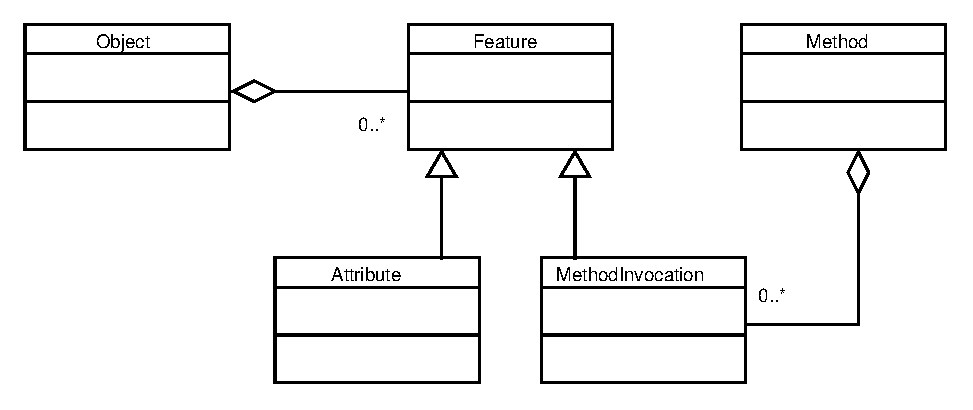
\includegraphics{observingMethods.eps}} \par}


\caption{Design for Observing Methods\label{Abb:observingMethods}}
\end{figure}

The point is, that not methods but method invocations are features observed
by invariants. A method invocation is a method together with a parameter sequence
suitable to invoke this method. 

Up to now, the implementation observes attributes only.


\subsection{Implementation}

Not all of these classes exist explicitly in the implementation. \emph{Class}
and \emph{Object} are provided by the user model already. \emph{Invariant} exists
only as an additional method \texttt{checkOclInvariant\_<name>} of its context
class. \emph{InvariantInstance} is an explicit class\footnote{
called a bit confusingly \texttt{tudresden.ocl.injection.lib.Invariant}.
} of the injection library. Finally \emph{Feature} is provided by the user model,
but cannot be referred as a single java object. (\texttt{java.lang.reflect.Field}
is a field of a class, not of an object.) Whenever a feature has to be referred,
it is represented by it's observer collection object, which sufficient for the
needs of this implementation.

Changes of object features are detected with polling. For each feature the ocl
injector adds a backup to the class. 

\begin{lyxcode}
class~Person\\
\{\\
~~int~age;\\
~~int~age\_oclbackup=age;\\
\}
\end{lyxcode}
Additionally there is a utility method added comparing each attribute to it's
backup. If there is a difference, the observers of the attribute are notified. 

\begin{lyxcode}
private~void~checkForChangedFeatures()\\
\{\\
~~if(age!=age\_oclbackup)\\
~~\{\\
~~~~age\_oclbackup=age;\\
~~~~//~notify~observers~of~age\\
~~\}

~
\end{lyxcode}
This method is called immediately before and after each method of the class.
If the attribute contains an object reference, the comparison tests object identity,
not object equality. This means, the \texttt{!=} operator is used as for basic
types and not the \texttt{equals()} method. For collections the backup stores
a hashcode\footnote{
see \texttt{tudresden.ocl.injection.Invariant.identityHashCode}.
} of the collection to avoid the overhead of maintaining a complete backup collection.


\chapter{Reverse Engineering\label{Sec:ReverseEngineering}}

Section \ref{Sec:element_type_tag} explained, how to store additional type
information of a java model in java documentation tags. This section discusses,
how to generate this information.

An interactive tool for injecting \texttt{@element-type} and \texttt{@key-type}
tags into the code using information obtained from the source code or dynamically
on run time.


\section{Static Information}

Information about element types may be derived from static properties of the
class, such as parameter types of methods and tags in doccomments. The following
example suggests some of these properties. 

\begin{lyxcode}
/{*}{*}\\
~~~All~employees~of~this~company.\\
~~~@see~\underbar{Person}\\
{*}/\\
Collection~employees;\\
~\\
boolean~isEmployee(\underbar{Person});\\
void~addEmployee(\underbar{Person});\\
void~removeEmployee(\underbar{Person});
\end{lyxcode}
An interactive tool should support the developer by presenting these properties
in a comfortable way. There should be a special indication, if several properties
suggest different element types.

Note, that the example above requires linguistic knowledge about plural and
singular form of nouns (employee here). This gets far more difficult, if identifiers
are not English.


\section{Tracing Dynamic Type Information}

\begin{itemize}
\item Enrich the code with tracing the object types inside collections.
\item compile and run the program (regression tests if available)
\end{itemize}

\chapter{Maintaining the OCL Compiler}

This chapter describes all major changes to Frank Fingers OCL compiler. This
includes bugfixes too, if they caused changes of internal or external interfaces.


\section{Using reflection in ReflectionFacade and ocl library}

\begin{enumerate}
\item Added polymorphism of operation parameters (ReflectionFacade.\-navigateParameterized
and OclAnyImpl.getFeature). This made ReflectionAdapter.getClassForType superfluous,
so removed.
\item Now its mandatory to provide a NameAdapter to the ocl library. Otherwise NullPointerExceptions
are thrown. The default functionality if no NameAdapter is given has been moved
into a separate NameAdapter (SimpleNameAdapter) which is used in ReflectionFacade
as well. 
\item Added a simplified form of qualified associations to ReflectionFacade and ocl
library. Simplification means, that there may be only one qualifier attribute.
Qualified associations are represented by java.util.Map. ReflectionAdapter.isMap.
\item New mapping beetween collections in OCL and Java conforming to JDK1.2. The special
handling of Vector is used for older code generators. (DefaultOclFactory.getOclRepresentationFor(Object)
and DefaultReflectionAdapter.getClassForType)

\vspace{0.3cm}
{\centering \begin{tabular}{|c|c|c|}
\hline 
Java (java.util)&
Ocl.TAKE\_VECTORS\_AS\_SET&
OCL\\
\hline 
\hline 
List&
-&
Sequence\\
\hline 
Vector&
false&
Sequence\\
&
true&
Set\\
\hline 
Set&
-&
Set\\
\hline 
Map&
-&
Set (qualified)\\
\hline 
\end{tabular}\par}
\vspace{0.3cm}

\end{enumerate}

\section{ocl lib}

\begin{enumerate}
\item removed \texttt{Ocl.STRICT\_CHECKING}, replaced exceptions by undefined values,
parameterized with the reason for the undefined value.
\item Ocl.Collection.setToRange makes an undefined collection (instead of throwing
an exception), if lower bound is greater than upper bound.
\item Ocl.to<OclType>(OclRoot) methods check for undefined arguments.
\end{enumerate}

\section{Typechecker}

\begin{enumerate}
\item added OclAny to TypeChecker (DefaultTypeFactory). 
\item Bugfix, removed TypeFactory.getClassifier - replaced all calls by TypeFactory.get
\end{enumerate}

\section{JavaCodeGenerator: \label{Sec:maintainJavaCodeGenerator}}

\begin{enumerate}
\item different meaning of Codefragments created for @pre expressions (TRANSFER, PREPARATION,
CODE), makes it easier and more flexible for different code injector tools.
compare to \cite{ff3} section 7.1.2, description of new behavior in section
\ref{Sec:codegeneration_result}, TODO comparison to Franks example
\item explicit package qualifier for ocl library is optionally prepended. Replaces
the import statement and therefore fulfills the corresponding requirement in
section \ref{Sec:injection_requirements}.
\end{enumerate}

\section{Silly Bugfixes}

\begin{enumerate}
\item JavaCodeGenerator: order on arrow
\item Basic.navigate: max{[}1{]}
\item DefaultOclFactory.getOclRepresentationFor(Object): dealing with Float and Double
\item OclCollection.setToRange: exchanged bounds in error condition
\end{enumerate}
\appendix

\chapter{Injector Tutorial}

This chapter describes, how to use the injector tool.

\listoffigures

\begin{thebibliography}{WK99}
\bibitem[FF00]{ff3}Frank Finger. Design and Implementation of a Modular OCL Compiler. Diplomarbeit.
TU-Dresden 2000. http://www-st.inf.tu-dresden.de/ocl/
\bibitem[WK99]{Warmer}Jos Warmer, Anneke Kleppe. The Object Constraint Language: Precise Modeling
with UML. Addison-Wesley, 1999.
\bibitem[UML]{UML}OMG Unified Modeling Language Specification, Version 1.3, June 1999.
\bibitem[OCL]{OCL}Object Constraint Language Specification. Chapter 7 in \cite{UML}.
\bibitem[JAVA]{JAVA}James Gosling, Bill Joy, Guy Steele. The Java Language Specification. Edition
1.0. August 1996.
\end{thebibliography}
\end{document}
